\chapter*{Użyte technologie}
Głównymi czynnikami decydującymi o doborze silnika były:
\begin{itemize}
	\item Prostota interakcji z kartą graficzną,
	\item Dobre narzędzia do debugowania kodu,
	\item Jakość i kompletność dokumentacji,
	\item Wydajność,
	\item Możliwość prostej implementacji interfejsu graficznego,
	\item Wcześniejsze doświadczenie,
	\item Szybkość kompilacji -- istotna przy częstych zmianach w kodzie.
\end{itemize}
\section*{Unity}
Unity to wieloplatformowy silnik autorstwa firmy Unity Technologies, którego głównym zastosowaniem jest tworzenie gier dwuwymiarowych i trójwymiarowych oraz symulacji. W porównaniu do podobnych narzędzi wyróżnia się prostotą obsługi, dużym naciskiem na edytory wizualne i zintegrowanym środowiskiem, które nie wymaga skomplikowanej konfiguracji. Wspiera wiele API graficznych (DirectX, OpenGL, Metal i Vulkan)\cite{UnityManualGraphicsApiSupport} pod wspólnym interfejsem. Dzięki temu użytkownicy silnika mogą w łatwy sposób tworzyć wersje swoich aplikacji na wiele platform, bez konieczności uciążliwego dostosowywania swojego kodu. Podobne uproszczenia dostępne są również w zakresie obsługi urządzeń wejścia (jak mysz, klawiatura, kontrolery, ekrany dotykowe), a także dźwięku. Na wspomnienie zasługuje również wbudowany edytor WYSIWYG\footnote{WYSIWYG (What You See Is What You Get) - ,,otrzymujesz to co widzisz''} interfejsu graficznego aplikacji. Silnik można też rozszerzać o własne narzędzia, na przykład graficzny edytor krzywych. Programować swoją aplikację można jedynie w języku C\texttt{\#}~\cite{ProgramminginUnity}. Interfejs edytora Unity przedstawiono na rysunku~\ref{fig:unity}.
\section*{Język C\texttt{\#}}
C\texttt{\#} to silnie i statycznie typowany, obiektowy język programowania zaprojektowany przez firmę Microsoft. Pozwala pisać kod z zachowaniem wszystkich założeń obiektowego paradygmatu programowania, czyli: abstrakcji, hermetyzacji, polimorfizmu i dziedziczenia. Mimo że C\texttt{\#} to język obiektowy, posiada wiele funkcji inspirowanych językami funkcyjnymi, które pozwalają m.in. bardzo łatwo dokonywać filtrowania, przekształcania czy sortowania kolekcji obiektów. Ułatwia to pisanie czytelnego, a przy tym zwięzłego, kodu. Pierwotnie kod C\texttt{\#} mógł być uruchamiany jedynie na systemie Windows. Zmieniło się to jednak w ostatnich latach dzięki środowiskom takim jak Mono oraz .NET Core i obecnie wspierane są inne systemy, takie jak Linux, macOS, iOS czy Android~\cite{Albahari2017}.
\begin{figure}[h!]
	\centering
	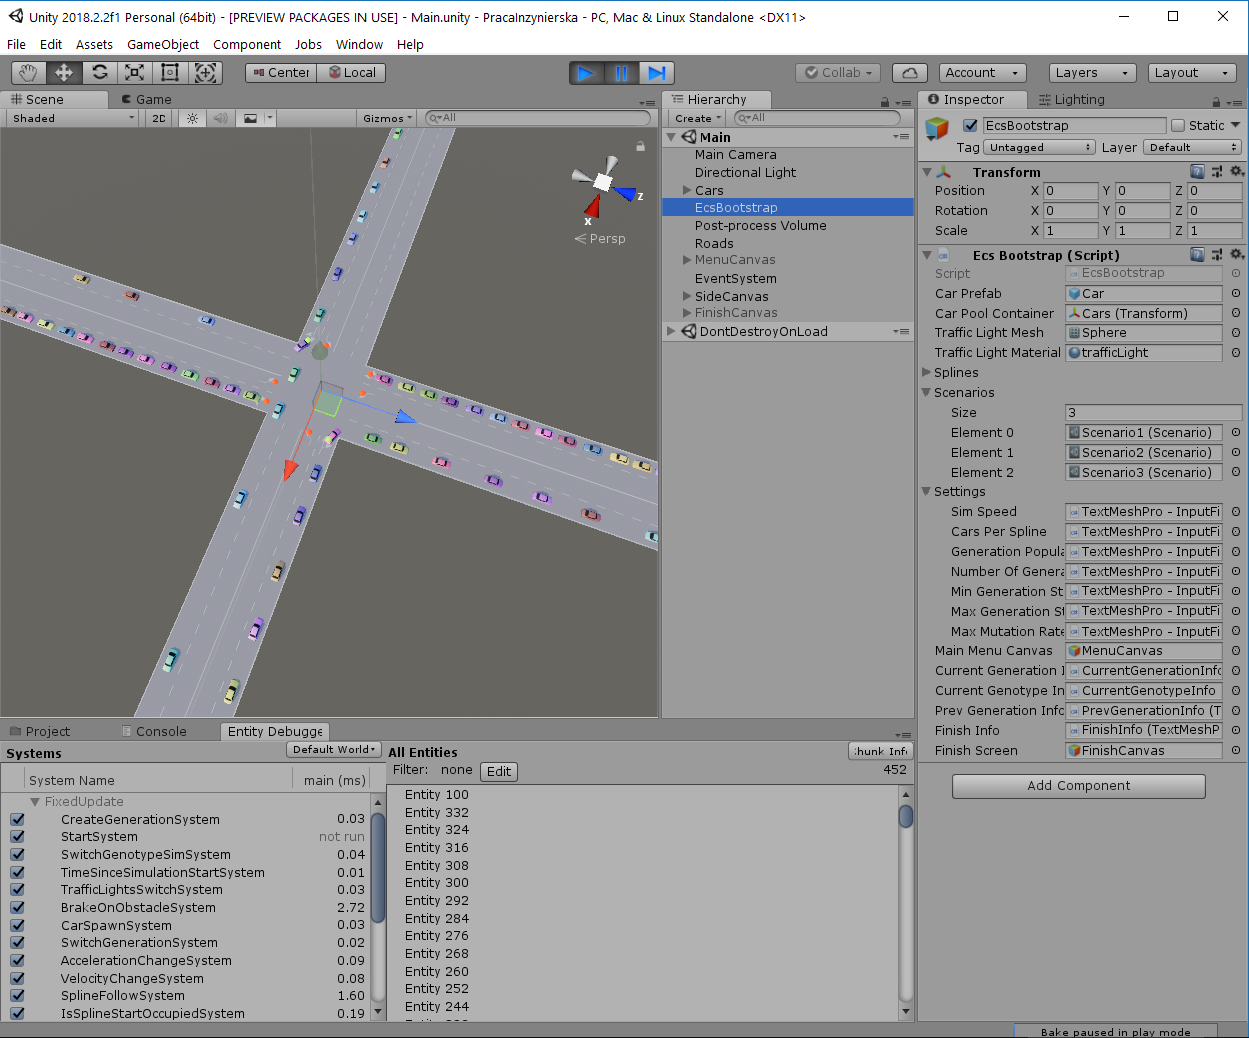
\includegraphics[width=1\linewidth]{unity}
	\caption[Interfejs edytora Unity]{Interfejs edytora Unity}
	\label{fig:unity}
\end{figure}
\section*{Inkscape}
Inkscape to darmowy program do tworzenia grafiki wektorowej. Tworząc w nim obrazy korzysta się z podstawowych kształtów takich jak elipsy, wielokąty, krzywe czy strzałki. Inkscape używa formatu Scalable Vector Graphics (SVG). Mimo że program opiera się na formacie wektorowym, plikiem wynikowym rysunku w tej pracy był obraz rastrowy, który można eksportować w dowolnej rozdzielczości. Decyzja ta wynika z ograniczeń w importowaniu grafik wektorowych w silniku Unity. Za użyciem Inkscape przemawiała przede wszystkim mnogość narzędzi i ustawień do tworzenia kształtów i wyrównywania ich położenia. Wygląd interfejsu programu przedstawiono na rysunku~\ref{fig:inkscape}. \\
W tej pracy został użyty do stworzenia grafiki skrzyżowania.
\begin{figure}
	\centering
	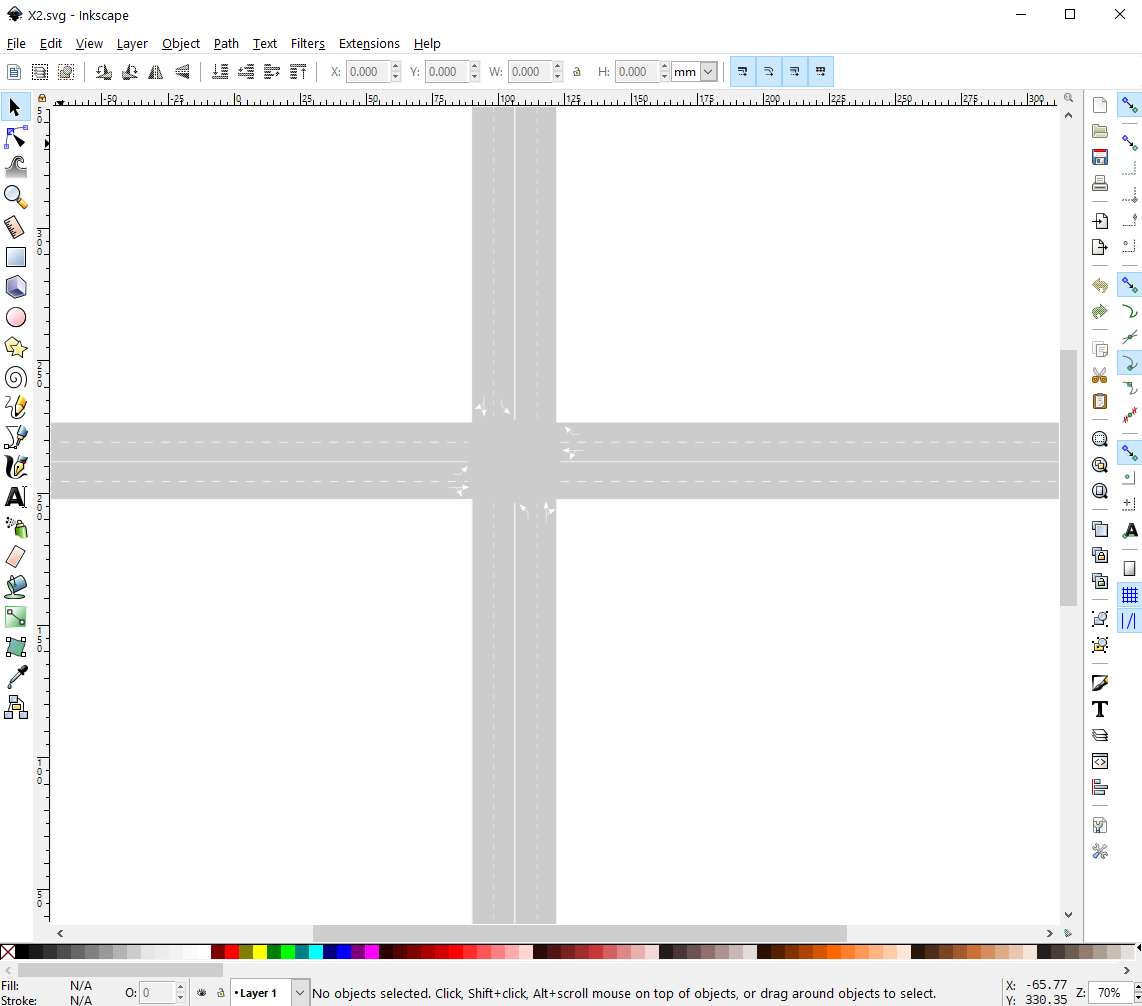
\includegraphics[width=1.0\linewidth]{inkscape}
	\caption[Interfejs programu Inkscape]{Interfejs programu Inkscape}
	\label{fig:inkscape}
\end{figure}
\section*{Blender}
Blender to darmowy program do tworzenia grafiki trójwymiarowej stworzony przez organizację Blender Foundation. Posiada narzędzia do modelowania, teksturowania, renderowania i animacji. Oprócz tego można z jego użyciem wykonywać proste symulacje fizyczne, a nawet zrealizować postprodukcję filmów. Niewątpliwie zaletą programu jest połączenie ogromnej liczby narzędzi w jeden pakiet. Dodatkowe atuty to dobra integracja z silnikiem Unity, wygoda użytkowania i wydajność. W tej pracy posłużył do wykonania trójwymiarowego modelu samochodu oraz ikony aplikacji. Interfejs Blendera przedstawia rysunek~\ref{fig:blender}.
\begin{figure}[h!]
	\centering
	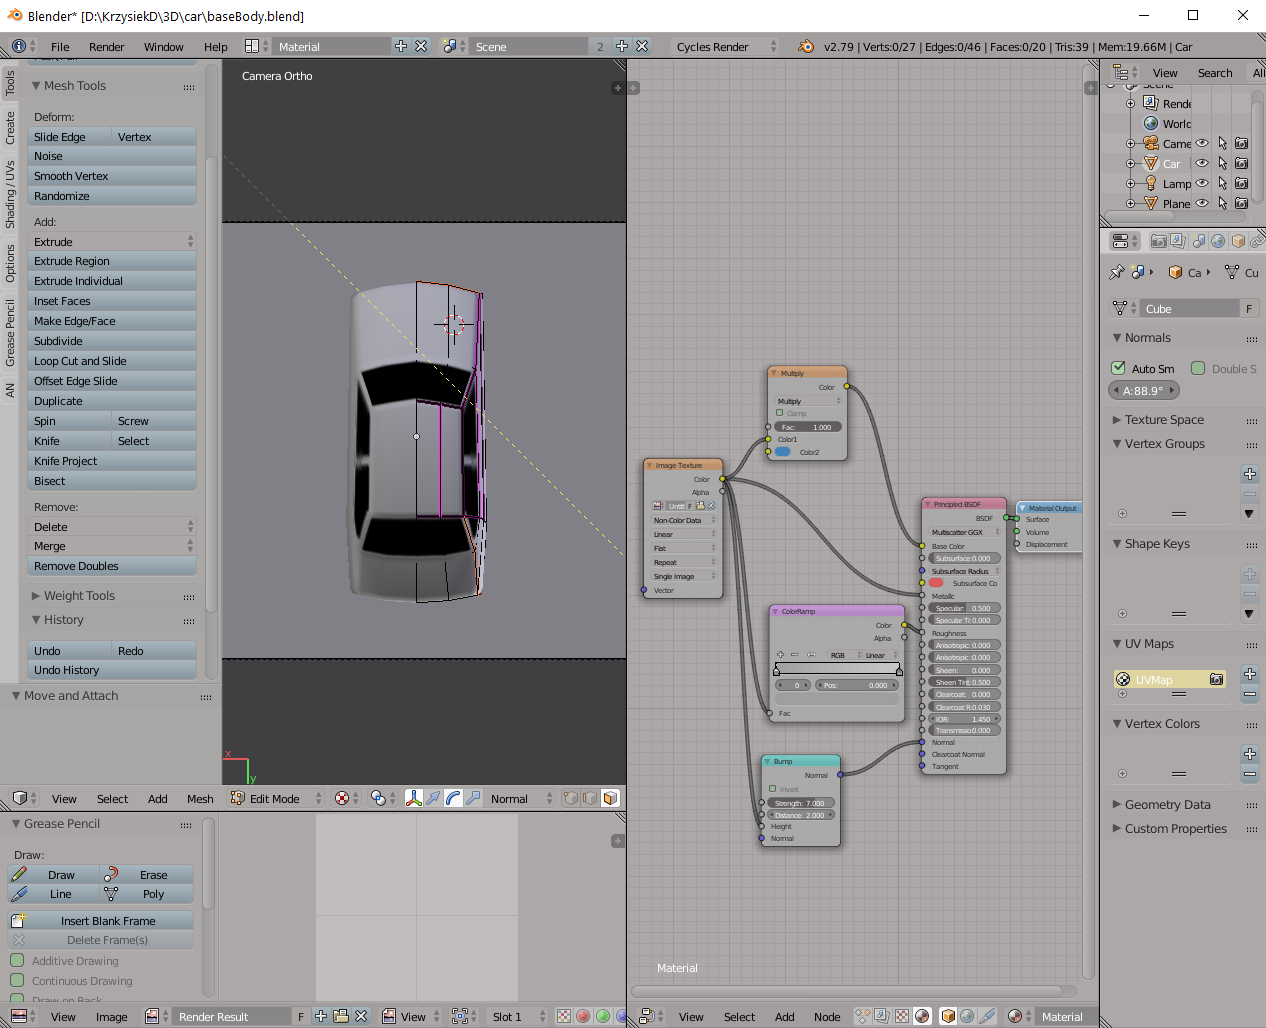
\includegraphics[width=1\linewidth]{blender}
	\caption[Interfejs programu Blender]{Interfejs programu Blender}
	\label{fig:blender}
\end{figure}

